\chapter{Comportamiento de cambio de carril}
\label{ch:lane-change-model}

El problema del cambio de carril determina cuándo y cómo realiza los cambios de carril un conductor en un momento determinado. A priori la intuición sobre el problema es que muchos de los factores determinantes no son medibles en el mundo real y/o en el entorno simulado (e.g. estados de humor, condición física, eventos fortuitos, etcétera).

En un trabajo anterior~\cite{CITA DEL ARTÍCULO DE LANE EXECUTION CUANDO NOS LO PUBLIQUEN} los autores tratamos de controlar muchos de estos factores dividiendo el problema en dos partes, la intención de cambio y la ejecución del cambio, fijando el primero de manera que los conductores sólo cambiaban de carril cuando se les ordenaba y permitiendo estudiar, de esta manera, cómo diferentes perfiles de conductores ejecutaban de diferente forma el cambio de carril y cómo este fenómeno es modelable.

En este trabajo se tratará de modelar, sin embargo, el proceso de cambio de carril como un todo, esto es, decidir en cada momento si cambiar a un caril (i.e. izquierda o derecha) o no hacerlo, a partir de las variables medibles del entorno real y simulado. El problema de ajuste será por tanto un problema de clasificación donde se tratará de maximizar el número de aciertos entre los cambios de carril realizados y el modelo a ajustar. Las técnicas que se han seleccionado para tratar el cambio de carril son las siguientes:

\begin{enumerate}
	\item \ac{mlp}. Los \acp{mlp}, más ahora en la época del \textit{deep-learning} son una de las técnicas más usadas para problemas de clasificación. En esta época del \textit{deep-learning} han aumentado su eficiencia varios ordenes de magnitud en capacidad de aprendizaje y, por tanto, en rendimiento a la hora de clasificar.
	\item \ac{cnn}. Otro de los grandes exponentes a la hora de clasificar, sobre todo trabajando con mapas de características $n$-dimensionales con las \acp{cnn}. Al representar la evolución temporal del entorno circundante como un espacio tridimensional, podemos aplicar esta técnica para la identificación de características de manera, supuestamente, más eficiente.
\end{enumerate}

Ambos modelos, al igual que ocurría con el modelo longitudinal, han sido entrenados ajustando sus parámetros con el algoritmo ADAM~\cite{kingma2014adam}. Las funciones de activación, sin embargo, varían, y por tanto la inicialización de las variables también\sidenote{
	La inicialización clásica, de valores uniformes en un intervalo pequeño alrededor de $0$ haría que la mitad de los valores cayesen por debajo de 0. Si la neurona tiene una función de activación de tipo \ac{relu}, el peso no se vería modificado, ya que su derivada será siempre $0$.
}.

En este caso, ambos modelos hacen uso de neuronas de activación de tipo \ac{relu}, salvo en la última capa que la activación es lineal. Para inicializar los pesos de las variables se hace uso del algoritmo Glorot~\cite{glorot2010understanding} (también denominado Xavier) debido a su mejor desempeño, sobre todo en redes con funciones de activación tipo \ac{relu}~\cite{glorot2011deep}\sidenote{
	Esta inicialización se basa en intentar mantener la misma desviación típica de gradientes en cada capa de la red. En~\cite{glorot2010understanding} determinan que ésta debe ser $\sigma^l = \frac{2}{\mathbf{card}(W^l_{in}) + \mathbf{card}(W^l_{out})}$, siendo $\mathbf{card}(W^l_{in})$ y $\mathbf{card}(W^l_{out})$ el número de entradas y de salidas de la capa, extrayendo posteriormente sus valores de una distribución aleatoria de la forma $X^l \sim \mathcal{N}(\mu=0,\sigma=\sigma^l)$
}.

Al tratarse además de un problema de clasificación donde las clases son mutuamente excluyentes, a la capa de salida de las redes se le ha aplicado una normalización\sidenote{
	La normalización usada ha sido la operación denominada softmax, definida como:
	\begin{equation}
		softmax(\vec{x})_i = \frac{e^{x_i}}{\sum_{j=1}^n e^{x_j}}
		\label{eq:softmax}
	\end{equation}
} para transformar el vector de salida en un vector de probabilidades, siendo el cambio de carril seleccionado la salida con el valor de probabilidad más alto.

Antes de pasar a la descripción de los modelos, queda hablar del sesgo existente en los datos de entrenamiento. Debido a la naturaleza el problema, el número de ejemplos existentes de cambios de carril es significativamente menor al existente de no cambios de carril. Este sesgo hace que los modelos se entrenen rápidamente para marcar todos los ejemplos como \enquote{no cambio}, dificultando el ajuste posterior hacia cambios a izquierda o derecha.

Por tanto, debido a que (i) las limitaciones de la máquina no nos permiten operar con los conjuntos completos en cada epoch y (ii) existe un sesgo hacia predicciones de \enquote{no cambio}, en cada uno de los epochs, se usará un batch para entrenar de tamaño $m = 6.000$ compuesto por una selección aleatoria de todos los ejemplos equidistribuida entre las clases de los ejemplos (esto es, aproximadamente $\frac{m}{3}$ para cada clase \enquote{cambio izda.}, \enquote{no cambio} y \enquote{cambio dcha.}).

\section{Descripción de los datasets}

Del conjunto de datos~\ref{tbl:main-variables} descrito en el capítulo~\nameref{ch:methodology} seleccionaremos aquellos indicadores de interés y generaremos un conjunto de entrenamiento y test para cada uno de los sujetos y un conjunto de entrenamiento y test para el total de conductores.

\subsection{Representación de los datos}

Las secuencias de las que se compone el conjunto de datos están compuestas, aparte de variables numéricas, de una representación del entorno del vehículo como nube de puntos. Los límites técnicos y la representación en sí implican dos problemas principales:

\begin{enumerate}
	\item Los modelos que utilizamos en esta tesis se basan en un número fijo de entradas, y la nube de puntos contiene un número variable de éstos, dependiendo del número de obstáculos y su distancia al origen.
	\item La nube de puntos se origina a través de un dispositivo mecánico que funciona con coordenadas esféricas a una resoluciones horizontal de \SI{0.2}{\degree}\sidenote{
		Funcionando a \SI{10}{\hertz}.
	} y vertical de \SI{2}{\degree}. Esto implica que la superficie del sector circular que no se cubre a largas distancias sea muy extenso, por lo que el espacio según nos alejamos del origen va siendo cada vez más diperso.
\end{enumerate}

Para el primer caso, se ha optado por representar el entorno como un mapa de profundidad, ilustrado en la Figura~\ref{fig:deepmap-example}. Un mapa de profundidad representa el entorno como una imagen de un sólo canal donde cada píxel representa la distancia a un sector esférico del espacio original.

\begin{figure}
	\centering
	
\includegraphics{deepness-map}
	\caption[Ejemplo de un mapa de profundidad]{Un ejemplo del mapa de profundidad asociado a la nube de puntos original\TODO{sacar un mapa de profundidad de los nuevos, porque se ven mejor}.}
	\label{fig:deepmap-example}
\end{figure}

Dado que el LIDAR describe el entorno de manera discreta con valores constantes de elevación y azimuth, se puede definir una biyección entre el conjunto de puntos original y los píxeles del mapa de profundidad, por lo que la información disponible en ambas es equivalente. Sin embargo, en nuestro caso no necesitamos una representación tan fiel del entorno porque:

\begin{itemize}
	\item La resolución horizontal produce un mapa de profundidad de $1800$ columnas. Esta resolución es extremadamente grande, y requeriría el uso de modelos con muchos parámetros, pudiendo caer fácilmente en un problema de \textit{over-fitting}.
	\item La apertura vertical del LIDAR genera puntos en planos que no son relevantes para el problema. Esto es, planos muy bajos que impactan en el vehículo o muy altos que no impactan con el entorno considerado de interés.
\end{itemize}

Por estas razones, los mapas de profundidad se generarán de una manera más compacta, usando una resolución horizontal de \SI{1}{\degree} y los seis canales que van desde los \SI{-7}{\degree} hasta los \SI{3}{\degree}, lo que nos da un mapa de profundidad con una resolución de $6 \times 360$ con un canal representando la distancia al punto de impacto más cercano contenido en el sector esférico que representa cada posición del mapa.

Para el segundo caso, se ha definido un radio de interés de \SI{25}{\meter}, ya que se ha considerado para el proceso de cambio de carril como un entorno lo suficientemente amplio para determinad un cambio de carril.

Con estos datos, los mapas de profundidad serán normalizados al intervalo $[0, 1] \in \mathbb{R}$ invertido, esto es, los valores mas cercandos al vehículo serán más próximos a 1 mientras que los valores más alejados estarán más próximos a 0.

\subsection{Generación artificial de datos}

Este problema de Los problemas con alta variabilidad de sus entradas suelen ser complejos y requerir de conjuntos de datos de tamaños bastante grandes para poder identificar patrones, como lo son por ejemplo los problemas de reconocimiento de imágenes.

En nuestro caso, el modelo de cambio de carril tiene como entrada una nube de puntos, la cual representa en un espacio de 3 dimensiones un conjunto muy limitado de puntos, con la dificultad añadida de que el \ac{lidar} tiene de base un error de \SI{3}{\cm}. Como el espacio sobre el que trabajar es tan complejo, se requerirían modelos con muchos parámetros, pero al disponer de pocos ejemplos, podríamos caer muy fácilmente en problemas de \textit{over-fitting}.

Por ello, se ha optado por realizar un proceso de generación de datos artificiales a partir de los datos existentes. De esta manera, ayudaremos al modelo a entrenar con casos similares y que de esta manera generalice mejor. La generación artificial se ha realizado sobre los datos recogidos en la ruta $R_1$, ya que es la que nos proporciona la información para entrenar el modelo y es por tanto en el único conjunto que cobra sentido este proceso. Concretamente hemos hecho uso de dos técnicas, primero un \textit{mirroring} sobre todas las filas del conjunto y diez aplicaciones de la técnica \textit{shaking} sobre el nuevo conjunto con los datos originales y simétricos.

La aplicación de estas técnicas requiere además que las nuevas porciones de datos generadas mantengan una coherencia temporal. Por tanto, aunque pertenezcan al mismo conjuntos de datos, cada uno se mantiene en una secuencia independiente.

A continuación se pasan a describir los procesos de generación de datos artificials introducidos previamente.

\paragraph{mirroring}

Se parte de la suposición de que los procesos cognitivos que producen determinados comportamientos (en nuestro caso, el cambio de carril) son los mismos independientemente de un cambio a la izquierda o hacia la derecha\sidenote{
	Es una suposición que en estudios sucesivos se puede tratar de refutar. Sin embargo, en el estadio actual de la investigación, nos parece razonable asumir que los procesos cognitivos en ambas situaciones son equivalentes.
}.

Por tanto, para cada fila generaremos una nueva nube de puntos a partir de una simetría respecto al plano XY (recordemos que el eje X determina el sentido del movimiento del vehículo). De esta manera, modificando las variables pertinentes\sidenote{
	Es decir, invirtiendo los cambios de carril y la distancia recorrible en carriles izquierdo y derecho.
}, de cada ejemplo obtenemos uno nuevo. En la figura~\ref{fig:mirroring-example} se ilustra un ejemplo de este proceso sobre una nube de puntos arbitraria dentro del conjunto de ejemplos.

La principal ventaja de esta aproximación es que es posible doblar el tamaño del conjunto de datos sin afectar añadir más ruido al existente en los mismos.

\begin{figure}[t]
	\centering
	\subfloat[]{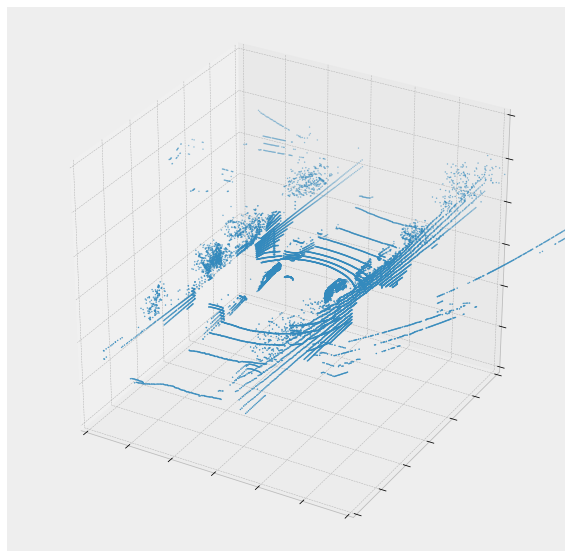
\includegraphics[width=.45\textwidth]{base-pointcloud}}\qquad
	\subfloat[]{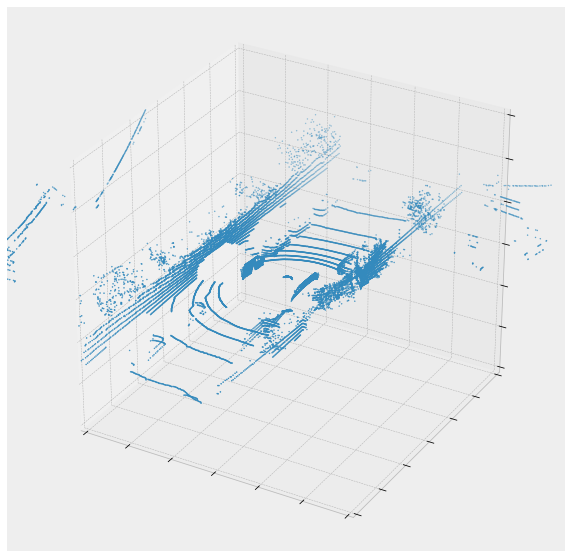
\includegraphics[width=.45\textwidth]{mirrored-pointcloud}}
	\caption[Ejemplo de la técnica de \textit{mirroring}]{Un ejemplo de una nube de puntos (a) original, y (b) tras aplicarle el proceso de mirroring. Para cada fila, tras un proceso de mirroring y una inversión de las variables simétricas en función de la conducción (cambio de carril y distancia recorrible) se genera una nueva fila válida para el conjunto de datos.}
	\label{fig:mirroring-example}
\end{figure}

\paragraph{shaking}

Esta técnica, a diferencia del \textit{mirroring} sí puede llegar a tener impacto en la precisión de los datos. Partiendo de una nube de puntos original\sidenote{
	Debido a que la aplicación iterativa de este proceso sobre la misma nube de puntos acumula los errores entre iteraciones haciéndola ininteligible.
}, se aplica un desplazamiento aleatorio $(\delta x, \delta y, \delta z)$ sobre cada punto tal y como se describe en~\cite{EL PAPER CUANDO NOS LO PUBLIQUEN}. La figura~\ref{fig:shaking-example} ilustra dos procesos de shaking con diferentes desplazamientos sobre la nube original mostrada en la figura~\ref{fig:mirroring-example}

\begin{figure}[b]
	\centering
	\subfloat[]{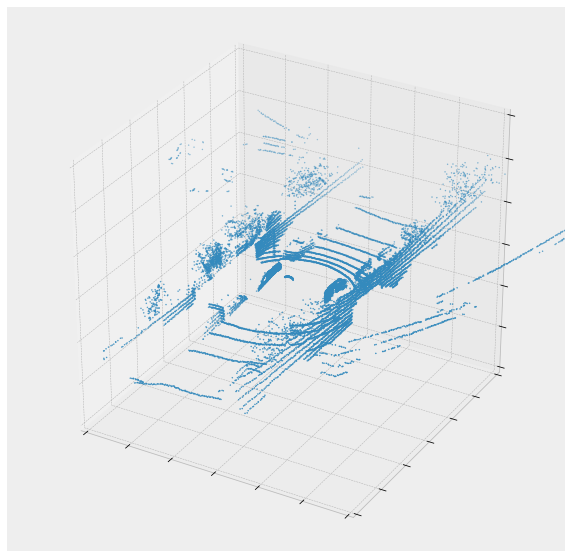
\includegraphics[width=.45\textwidth]{shaken-pointcloud-05}}\qquad
	\subfloat[]{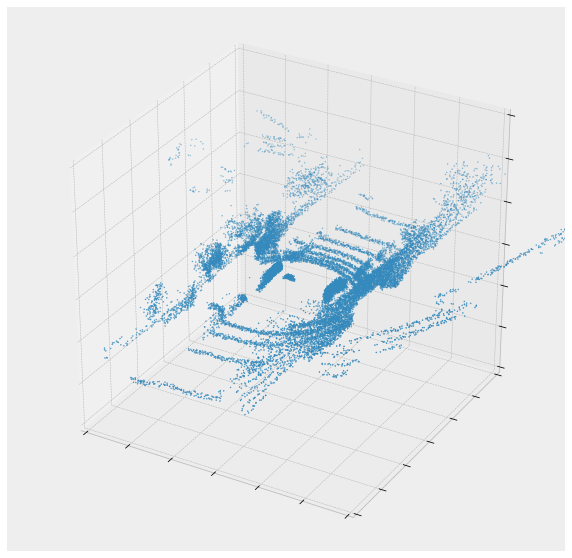
\includegraphics[width=.45\textwidth]{shaken-pointcloud-2}}
	\caption[Ejemplo de la técnica de \textit{shaking}]{Un ejemplo de dos nubes de puntos tras pasar el proceso de shaking con un desplazamiento $(\delta x, \delta y, \delta z)$ de (a) $(0.05, 0.05, 0.05)$ y de (b) $(0.2, 0.2, 0.2)$ sobre la nube de puntos original. Para cada fila, tras un proceso de shaking disponemos de una nueva fila ligeramente diferente de la original, añadiendo ruido y, presumiblemente, generalización al modelo tras el entrenamiento.}
	\label{fig:shaking-example}
\end{figure}

Las especificaciones técnicas del \ac{lidar} usado en los experimentos garantizan un error por debajo de los \SI{3}{\cm} de radio, por lo que un desplazamiento aleatorio para cada punto menor o igual que este valor no añadiría más ruido del existente. Sin embargo, en el experimento se ha optado sin embargo por aplicar un desplazamiento de $\delta x = \delta y = \delta z = 0.05m$ en cada eje, ligeramente superior al proporcionado por el lidar. De esta forma se pretende la incorporación de ruido sobre el entorno original para aumentar la capacidad de generalización del modelo\sidenote{
	La intuición de este proceso
}.

\subsection{Incorporación de información temporal}

Las \ac{cnn} son también redes que funcionan con un esquema \textit{feed-forward}, y por tanto tenemos el mismo inconveniente que vimos en el anterior capítulo acerca de mantener una noción temporal en nuestros modelos. En el caso del modelo longitudinal, se consigue este efecto incluyendo variables derivadas de la posición (i.e. velocidad y aceleración). Para el caso del entorno circundante hay que realizar un proceso similar.

En cada una de las filas poseemos una representación del entorno en forma de mapa de profundidad que describe el entorno, por lo que al modelo le alimentaríamos únicamente con la situación en un instante $t$ de tiempo. Esto no ayuda al modelo a descubrir patrones temporales como la velocidad o la aceleración puesto que no tiene información de eventos anteriores. Para solventar esta limitación, los conjuntos de datos serán transformados para que se alimenten con una ventana temporal de parámetros de entrada.

\begin{figure}[t]
	\centering
	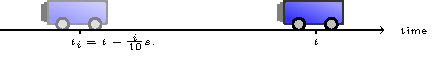
\includegraphics{explanation-of-data-frequency}
	\caption[Momento $t_i$en el conjunto de datos]{Un momento $t_i$ se define como el estado en el que se encontraba el vehículo en $t - \frac{i}{10}s$. Por tanto, $t_0$ es el momento actual.}
	\label{fig:moments-illustration}
\end{figure}

Comenzaremos definiendo el \textit{momento} $t_i$ como aquel ejemplo situado a $t - \frac{i}{10}s$ en el pasado (ver Figura~\ref{fig:moments-illustration}). Los momentos que se tendrán en cuenta en los datasets finales serán $t_0$, $t_10$, $t_20$, correspondientes al momento actual, \SI{1}{\second} anterior y \SI{2}{\second} anteriores respectivamente. Estos valores no son arbitrarios, sino que se han elegido de acuerdo a los experimentos realizados en~\cite{EL PAPER CUANDO NOS LO PUBLIQUEN}\sidenote{
	Dichos experimentos se corresponden con el proceso de ejecución de cambio de carril, donde se asume que la maniobra involucra al córtex visual y al córtex prefrontal. Estos procesos cognitivos tienen un tiempo de respuesta de entre \SI{0.2}{\second}, \SI{1.2}{\second}~\cite{buzsaki2012temporal}, por lo que es comprensible que la ventana temporal elegida sea aceptable. Además, al incluir tres momentos temporales, es posible que el modelo reconozca una intuición de la velocidad, la aceleración e incluso el \textit{jerk} a partir de imágenes estáticas. 
}.

Tras este ajuste, los conjuntos de datos están finalizados. Sus propiedades quedan descritas en la Tabla~\ref{tbl:lc-datasets-description}.

\begin{table}
	\caption[Descripción de los conjuntos de datos]{Descripción de los conjuntos de datos para el entrenamiento de los modelos.}
	\label{tbl:lc-datasets-description}
	\begin{tabular}{ccccc}
		\toprule
		Nombre & Entradas & Salidas & Tamaño (training) & Tamaño (test) \\
		\midrule
		$LC_{S_1}$ & $8653$ & $3$ & $68991$ & $2058$ \\
		$LC_{S_2}$ & $8653$ & $3$ & $84811$ & $2887$ \\
		$LC_{S_3}$ & $8653$ & $3$ & $82061$ & $2891$ \\
		$LC_{S_A}$ & $8653$ & $3$ & $248933$ & $7836$ \\
		\bottomrule
	\end{tabular}
\end{table}

\section{Modelo \ac{mlp}}

Los entrenamientos han sido realizados sobre diferentes topologías, siendo las más representativas las descritas en la tabla~\ref{tbl:lc-mlp-architectures}.

En lugar de intentar maximizar la cantidad de aciertos o minimizar el número de falsos positivos o negativos, el error que se ha tratado de minimizar es la entropía cruzada, concepto del cual hablamos anteriormente en el capítulo~\nameref{ch:sota-ci}. Este indicador es mucho más eficiente a la hora de trabajar con problemas de clasificación. Sin embargo, de cara a mostrar resultados en la tesis, el valor de ésta no ofrece información relevante más allá de \enquote{si decrece es bueno}. Por ellos se ofrecerán los valores de precisión y matrices de confusión que son más acordes con el problema en cuestión.

\begin{table}[t]
	\caption[Resumen de las arquitecturas \ac{mlp} para el modelo de cambio de carril]{Resumen de las arquitecturas de \ac{mlp} para el modelo de cambio de carril. La posición de cada número de la topología indica la capa, siendo su valor el número de nodos (neuronas) que incluye dicha capa. Las arquitecturas seleccionadas en esta tabla son aquellas consideradas relevantes tras un proceso manual de ensayo y error.}
	\label{tbl:lc-mlp-architectures}
	\begin{tabular}{ccccccc}
		\hline
		\multirow{2}{*}{Nombre} & \multirow{2}{*}{Topología} & \multirow{2}{*}{Epochs} & \multirow{2}{*}{Dropout} & \multicolumn{3}{c}{Precisión}  \\
		& & & & Training & Validation & Test \\ \hline
		$MLP_1$ & $64, 64$              & $10^5$ & $0.1$ & $0.33$ & $0.33$ & $0.33$ \\
		$MLP_2$ & $1024, 512, 128$      & $10^5$ & $0.1$ & $0.33$ & $0.33$ & $0.33$ \\
		$MLP_3$ & $1024, 512, 256, 128$ & $10^5$ & $0.1$ & $0.33$ & $0.33$ & $0.33$ \\ \hline
	\end{tabular}
\end{table}

La figura~\ref{fig:lc-mlp-accuracy-comparison} nos muestra la evolución de la precisión alcanzada por los modelos a lo largo del entrenamiento, tanto en entrenamiento como en el posterior test.

\begin{figure}
	\centering
	\subfloat[]{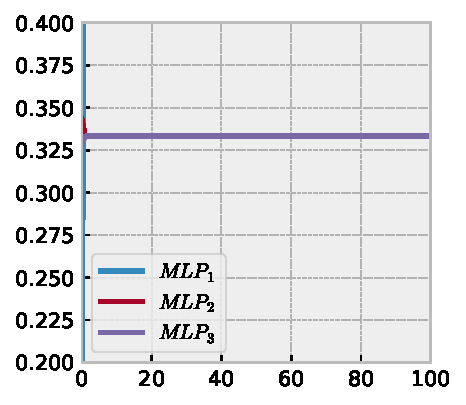
\includegraphics[width=.45\textwidth]{lc-mlp-acc-all-training-and-validation-detail}}\qquad
	\subfloat[]{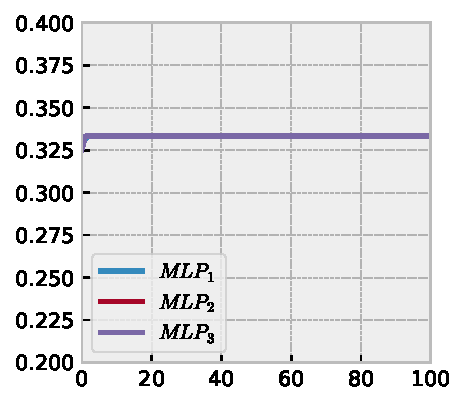
\includegraphics[width=.45\textwidth]{lc-mlp-acc-all-test-detail}}
	\caption[Comparación de las precisiones alcanzadas por los modelos de tipo \ac{mlp}]{Comparación de las precisiones alcanzadas por los modelos de tipo \ac{mlp}.}
	\label{fig:lc-mlp-accuracy-comparison}
\end{figure}

Cada una de las redes se ha entrenado durante $10^5$ epochs. A la vista de los resultados, la capacidad de predicción de este tipo de redes con el conjunto de datos propuesto no supera el valor de predecir de forma aleatoria\sidenote{Los ejemplos le son propuestos de forma equiprobable, por lo que al ser $3$ clases, la probabilidad de acerta de manera aleatoria es de $\frac{1}{3}$.}, por lo que el uso de~\ac{mlp} aquí es descartado completamente.

\section{Modelo \ac{cnn}}

Las arquitecturas de los modelos que mejores resultado han arrojado tras las pruebas se describen en la tabla~\ref{tbl:lc-cnn-architectures}.

\begin{table}[b]
	\caption[Resumen de las arquitecturas \ac{mlp} para el modelo longitudinal]{Resumen de las arquitecturas de \ac{mlp} para el modelo longitudinal. La posición de cada número de la topología indica la capa, siendo su valor el número de nodos (neuronas) que incluye dicha capa. Las arquitecturas seleccionadas en esta tabla son aquellas consideradas relevantes tras un proceso manual de ensayo y error.}
	\label{tbl:lc-cnn-architectures}
	\begin{tabular}{ccccccc}
		\hline
		\multirow{2}{*}{Nombre} & \multirow{2}{*}{Topología} & \multirow{2}{*}{Epochs} & \multirow{2}{*}{Dropout} & \multicolumn{3}{c}{RMS}      \\
		&                            &                         &                          & Training & Validation & Test \\ \hline
		$CNN_1$ & $7, 16, 1$                 & $10^5$                  & $0.1$                    & $0.052741$      & $0.057301$        & $0.059253$  \\
		$CNN_2$ & $7, 8, 4, 1$               & $10^5$                  & $0.1$                    & $0.056341$      & $0.061951$        & $0.056607$  \\
		$CNN_3$ & $7, 16, 8, 1$              & $10^5$                  & $0.1$                    & $0.046404$      & $0.051878$        & $0.059681$  \\ \hline
	\end{tabular}
\end{table}

La descripción de los parámetros de las arquitecturas es la siguiente:

\begin{itemize}
	\item \textbf{$cF$-$W$-$H$-$x$}. Esta nomenclatura se corresponde con una capa de convolución de $F$ filtros donde cada uno es tiene un tamaño de $W \times H$. $x$ puede tomar el valor $v$ (de \textit{valid}) o $s$ (de \textit{same}), dependiendo de si se desea que el filtro se limite a las dimensiones de la entrada o si por el contrario se prefiere que sobrepase los límites para que las convoluciones den como resultado una salida del mismo tamaño que la entrada original, respectivamente.
	\item \textbf{$dN$-$r$}. Esta capa se corresponde a las capas \textit{fully-connected} que realizan trabajan sobre el espacio de las características extraídas tras la extracción realizada en las convoluciones. En esta nomenclatura, $N$ se corresponde con el número de neuronas que tiene la capa y $r$ con la tasa de dropout aplicada a sus neuronas.
\end{itemize}

Existen una serie de particularidades del proceso de entrenamiento que hay que destacar. La primera y principal es la modificación de la arquitectura básica de una \ac{cnn} para atender a variables que no obedecen al esquema de mapa $n$-dimensional. Una \ac{cnn} basa su funcionamiento en una fase de extracción de características seguida de una fase de inferencia sobre las características extraídas de la imagen. En nuestro caso, sin embargo, necesitamos alimentar a la red con más información.

La decisión tomada ha sido entender estas variables (distancia circulable, distancia a siguiente semáforo y estado de siguiente semáforo) como características del modelo ya extraídas. Para ello, al alimentar el modelo, los mapas de profundidad y estas variables son separados al comenzar el entrenamiento. Los mapas de profundidades se pasan por el flujo normal de funcionamiento y una vez se han extraído las características de estos mapas se combinan con las variables para continuar con el flujo normal (ver Figura~\ref{fig:modification-of-cnn-to-work-with-variables})

\begin{figure}
	\centering
	\missingfigure[figheight=3cm]{Esquema donde se ve el flujo que siguen el deepmap y las variables dentro de la modificación de la red de convolución.}
	\caption[Esquema de modificación de \ac{cnn} para incluír características no espaciales]{Esquema de modificación de \ac{cnn} para incluír características no espaciales. Las variables se separan al principio de la convolución para que éstas trabajen con las imágenes. Una vez este proceso se ha completado, las características de las imágenes y las variables de entrada separada se vuelven a continuar para continuar el flujo normal de funcionamiento.}
	\label{fig:modification-of-cnn-to-work-with-variables}
\end{figure}

La siguiente modificación ha sido la alteración del mapa de profundidad justo al comienzo de la alimentación. Al ser los mapas de profundidad una representación cilíndrica de las distancias, el extremo izquierdo y el derecho de la imagen son, en realidad, un punto de corte donde las convoluciones perderán información. Para evitar esta limitación, las imágenes con las que se alimenta la red son aumentadas artificialmente en sus bordes con el extremo contrario de la imagen (ver Figura~\ref{fig:deepmap-augmentation-in-cnn}), para que la convolución opere sobre la información que de otro modo se perdería.

La última modificación es la de la aplicación de una tasa de aprendizaje adaptativa al proceso de entrenamiento. Esta adaptación puede basarse en muchos factores, pero en nuestro caso la tasa se basa en una disminución suave de un valor máximo a un valor mínimo de manera que en los primeros estadios del entrenamiento la tasa sea suficientemente alta como para converger rápidamente a zonas de interés, pero que a la vez, según el entrenamiento avanza, se eviten los problemas de saltos alrededor de mínimos. La tasa de aprendizaje en cada \textit{epoch} quedará determinada por la siguiente ecuación:

\begin{figure}[t]
	\centering
	\missingfigure[figheight=3cm]{Esquema donde se vea o que hago con la imagen al alimentar de poner parte de la izquierda en la derecha y viceversa..}
	\caption[Aumentación artificial de los extremos del mapa de profundidad]{Aumentación artificial de los extremos del mapa de profundidad. Para no perder información que puede ser relevante, los mapas se aumentan artificialmente al alimentar a la red, de tal manera que a los extremos izquierdo y derecho se les aumenta con parte de los extremos derecho e izquierdo con un número de píxeles igual a la mitad del tamaño horizontal del los filtros que los recorrerán.}
	\label{fig:deepmap-augmentation-in-cnn}
\end{figure}

\begin{equation}
    \alpha_i = \alpha_{min} + (\alpha_{max} - \alpha_{min}) \cdot e^\frac{i}{\alpha_d}
	\label{eq:learning-rate-decay}
\end{equation}

Donde $\alpha_i$ será la tasa de aprendizaje a aplicar en el \textit{epoch} $i$, $\alpha_{min}$ y $\alpha_{max}$ la cota inferior y superior que tomará la tasa de aprendizaje y $\alpha_d$ la tasa de decrecimiento. En la Figura~\ref{fig:learning-rate-decay} se ilustra la gráfica de la función usada para entrenar las arquitecturas de esta sección.

\begin{marginfigure}
	\centering
	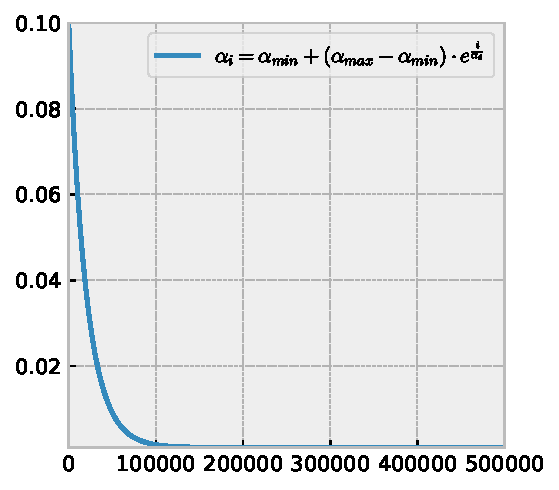
\includegraphics[width=\textwidth]{lc-learning-rate-decay}
	\caption[Gráfica de la tasa de aprendizaje adaptativo por epoch usada para entrenar \ac{cnn}]{Gráfica de la tasa de aprendizaje adaptativo por epoch usada para entrenar \ac{cnn}. En nuestros entrenamientos, los valores de los parámetros son $\alpha_{min} = 0.1$ y $\alpha_{max} = 0.001$ y $\alpha_d = 20000$.}
	\label{fig:learning-rate-decay}
\end{marginfigure}

Un último apunte antes de pasar a mostrar las gráficas de los entrenamientos. No se ha incluido ninguna capa de \textit{pooling} en las arquitecturas, sino que se ha preferido usar las capas de convolución sin añadir padding para ese efecto, tal y como proponen en~\cite{howard2017mobilenets}.

La evolución de la precisión a lo largo del entrenamiento para las diferentes arquitecturas se muestra en la Figura~\ref{fig:lc-cnn-training-validation-test-comparison}.

\begin{figure}[b]
	\centering
	\subfloat[]{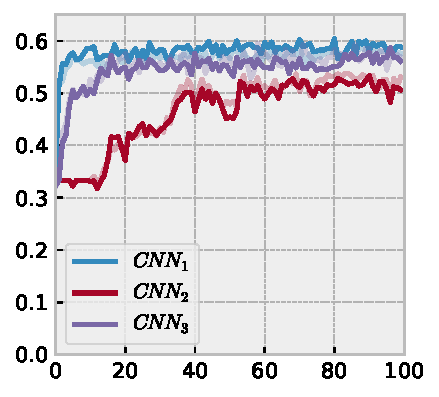
\includegraphics[width=.45\textwidth]{lc-cnn-acc-all-training-and-validation-detail}}\qquad
	\subfloat[]{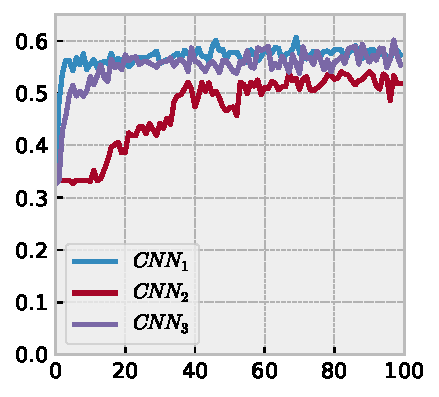
\includegraphics[width=.45\textwidth]{lc-cnn-acc-all-test-detail}}
	\caption[Comparación de las precisiones alcanzadas por los modelos de tipo \ac{mlp}]{Comparación de las precisiones alcanzadas por los modelos de tipo \ac{cnn}.}
	\label{fig:lc-cnn-training-validation-test-comparison}
\end{figure}

Se puede observar que se ha necesitado una red relativamente grande para superar el límite impuesto por la clasificación aleatoria. Esto contrasta con los resultados obtenidos en~\cite{EL PAPER PARA CUANDO NOS LO PUBLIQUEN}, donde los valores de clasificación eran mucho más altos. La razón por la que se intuye esta disparidad de datos es que es precisamente la operación de \textbf{decisión de cambio de carril} la que es más compleja de modelar, a diferencia de la de \textbf{ejecución de cambio de carril}, en la que esta decisión está ya tomada.

Probablemente con otra serie de variables se pueda aumentar la precisión de estos modelos, pero en este experimento estamos limitados al conjunto de variables observables en los entornos real y de simulación.

\section{Comparación entre modelos}

En este caso, las de las dos técnicas propuestas, la de \acp{mlp} ha sido descartada completamente al ser sus clasificación iguales a la de la selección aleatoria. Por tanto, el modelo que usaremos será el $CNN_2$, ya que es la única arquitectura que supera este límite.

En la figura~\ref{fig:lc-cnn-model-confussion-matrix} se expone la matriz de confusión asociada a esta arquitectura para los valores existentes en el conjunto de test.

\begin{figure}
	\centering
	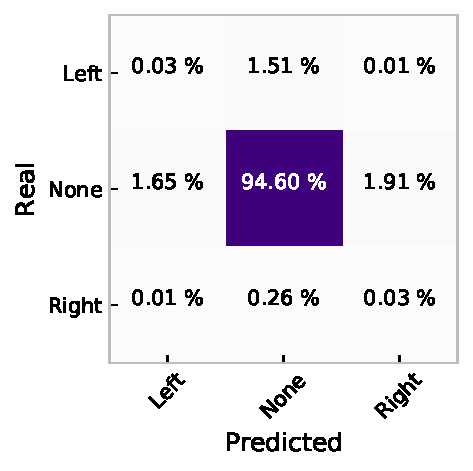
\includegraphics[width=.6\linewidth]{lc-cnn-model-confussion-matrix}
	\caption[Matriz de confusión del conjunto de test para \ac{cnn}]{Matriz de confusión del conjunto de test para \ac{cnn}.}
	\label{fig:lc-cnn-model-confussion-matrix}
\end{figure}
